\documentclass{article}
\usepackage{graphicx} % Required for inserting images
\usepackage{hyperref}
\hypersetup{
    colorlinks=true,
    linkcolor=blue,
    filecolor=magenta,      
    urlcolor=cyan,
    pdftitle={Overleaf Example},
    pdfpagemode=FullScreen,
    }

\urlstyle{same}


\title{Causal Inference Assignment}
\author{Parth Gupte}
\date{April 2024}

\begin{document}

\maketitle

\section{Q1 and 2}
Check handwritten PDF.\\
Also handed on paper in person.
\section{Q3}
\subsection{a) Exploratory Data Analysis}
After exploratory data analysis we find that the data comes from the same distribution for both treatment and control groups for all variables.\\
To do this we first plot the probability distributions of the columns in the form of a histogram and overlap the histogram for each 
columns for treatment and control groups.\\
\begin{figure}
    \centering
    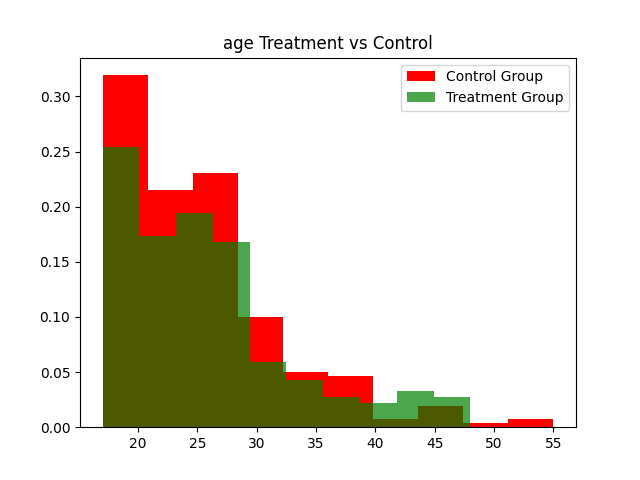
\includegraphics[width = 15 cm]{../age_cts_hist_plot.png}
\end{figure}

\begin{figure}
    \centering
    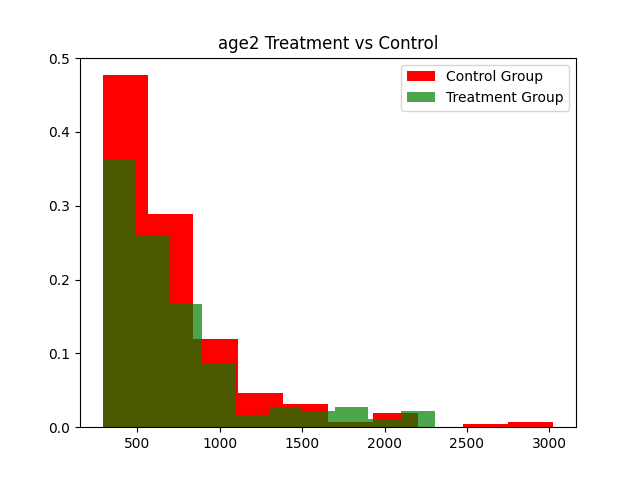
\includegraphics[width = 15 cm]{../age2_cts_hist_plot.png}
\end{figure}


\begin{figure}
    \centering
    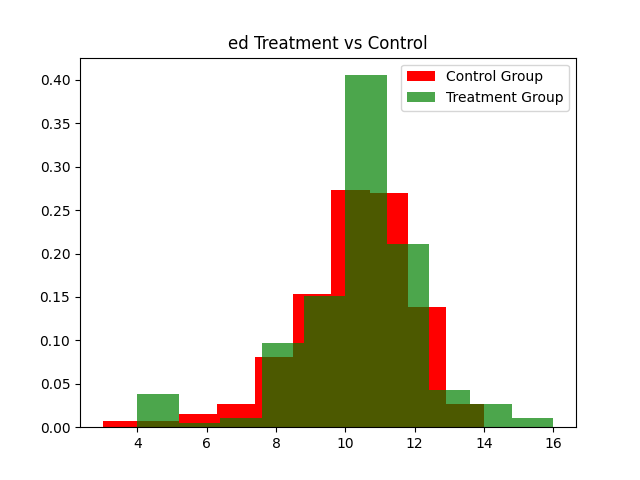
\includegraphics[width = 15 cm]{../ed_cts_hist_plot.png}
\end{figure}

\begin{figure}
    \centering
    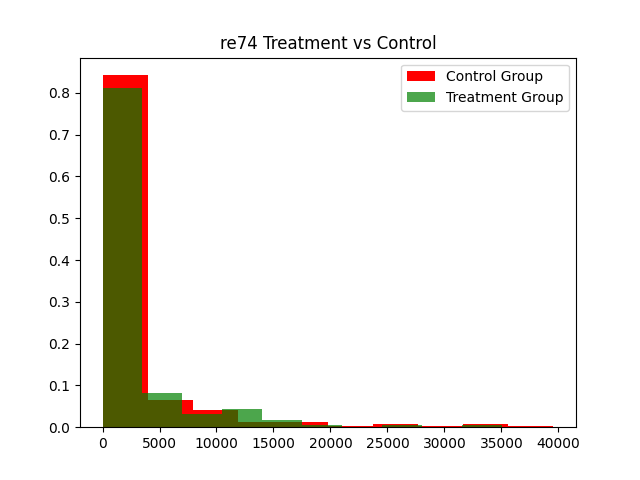
\includegraphics[width = 15 cm]{../re74_cts_hist_plot.png}
\end{figure}

\begin{figure}
    \centering
    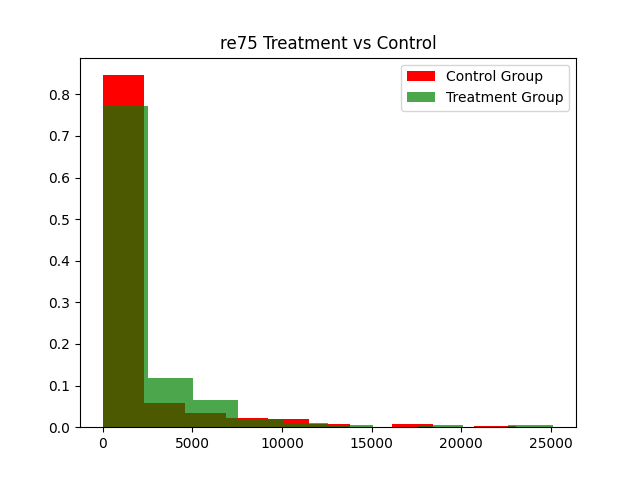
\includegraphics[width = 15 cm]{../re75_cts_hist_plot.png}
\end{figure}
\clearpage

As we can see for all of the variable the distributions look similar.
Now we use statistical tests to estimate the difference between these.\\

\subsubsection{Continous Variables}
For continous variables we use the students t-test to see if the means 
of the distributions are significantly different or not.\\
Here is what we obtain:\\
\begin{verbatim}
Column age has T-statistic value = 1.116614928783765 with p-value = 0.2647642688056856
Hence we cannot say that the distributions are diffrent with significance (<0.05)

Column re74 has T-statistic value = -0.022175136958298255 with p-value = 0.9823182350488567
Hence we cannot say that the distributions are diffrent with significance (<0.05)

Column re75 has T-statistic value = 0.8746214935780514 with p-value = 0.3822538041052975
Hence we cannot say that the distributions are diffrent with significance (<0.05)

Column age2 has T-statistic value = 0.9694696864328992 with p-value = 0.3328398944498051
Hence we cannot say that the distributions are diffrent with significance (<0.05)

Column ed has T-statistic value = 1.4958255190965968 with p-value = 0.13541116716943868
Hence we cannot say that the distributions are diffrent with significance (<0.05)
\end{verbatim} 

\subsubsection{Binary Variables}
For binary variables we use the chi-square test to check is the categorical
distributions are significantly different.\\
Here is what we obtain:\\
\begin{verbatim}
Column black as chi-sq value = 0.10662384969179997 with p-value = 0.7440210684680046
Hence we cannot say that the distributions are diffrent with significance (<0.05)
    
Column hisp as chi-sq value = 2.5705628867929904 with p-value = 0.10886898726859187
Hence we cannot say that the distributions are diffrent with significance (<0.05)
    
Column married as chi-sq value = 0.7277914114738451 with p-value = 0.39360001605637096
Hence we cannot say that the distributions are diffrent with significance (<0.05)
    
Column nodeg as chi-sq value = 9.41953941767863 with p-value = 0.0021468543756801464
Hence the distributions are the same with significance (<0.05)
\end{verbatim}
\clearpage

\subsection{b) Regression Analysis}
Next we perform linear regression on both the NSW dataset and
the CPS dataset, predicting the Earnings in 1978 (re78) based on
all the other variables.\\
Here were the results:\\
\begin{verbatim}
Model Coefs for NSW linear regression model:
{'treat': 1675.86237707045, 
'age': 141.7305740712043, 
'ed': 385.0161271012323, 
'black': -2155.6413034136403, 
'hisp': 187.26272427409285, 
'married': -184.89434030167712, 
'nodeg': -55.544821817317654, 
're74': 0.08147524244690274, 
're75': 0.05081520903056003, 
'age2': -1.4353216616441316, 
'intercept': -307.01194195694006}

Model coefs for CPS linear regression model:
{'treat': 0.0, 
'age': -252.04850736152875, 
'ed': 166.5983024477533, 
'black': -773.8794130598889, 
'hisp': -168.2285611161221, 
'married': 244.1442902105978, 
'nodeg': 330.6765477182316, 
're74': 0.2988692873561547, 
're75': 0.46995885500493273, 
'age2': 2.0408054257313957, 
'intercept': 7908.362295098289}

\end{verbatim}

\subsection{c) Matching through Propensity Score}
\subsubsection{Calculate Propensity Score}
We perform logistic regression, with treatment variable as the
dependent variable and all the other columns, other than re78 as the predictors
since re78 is an effect of treatment variable.\\
Here is the logitic model we obtain for calculating the Propensity
score:\\
\begin{verbatim}
Model Coefs for propensity score model:
{'age': -0.021718495698239637, 
'ed': -0.013541674687343404, 
'black': -0.0010854880038832747, 
'hisp': -0.0008041072459307032, 
'married': 0.00020745846105355112, 
'nodeg': -0.0029588755215886027, 
're74': -1.8443713277604196e-05, 
're75': 4.548966676852774e-05, 
'age2': 0.0004956004644433062, 
'intercept': -0.0016417668379095835}
\end{verbatim}
\clearpage

\subsubsection{Matching Method}
First we plot the propensity scores of the treatment group and
control group on a histogram to compare there values.\\
Here is the plot:\\
\begin{figure}[h]
    \centering
    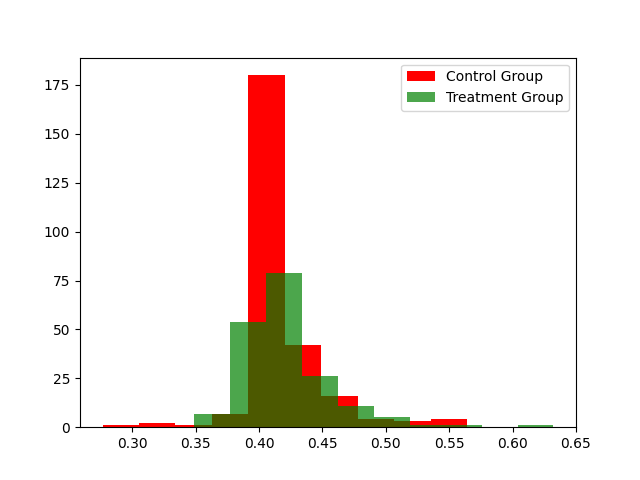
\includegraphics[width = 15 cm]{../treatmentvscontrol_common_base.png}
\end{figure}

So we can see that they do have a common support ranging from 
around 0.35 to 0.50.\\
\clearpage
Now we figure out the matchings between the control and treatment group.
Since we are to match every treatment point to one control point 
and repetition is allowed.\\
We follow the following algorithm:\\
\begin{enumerate}
    \item Choose point in treatment data
    \item Get its propensity score
    \item Iterate over all points in control group, and using a distance metric find the point in control whose propensity score is closest to the point in treatment
    \item Match this control point to the choosen treatment point
    \item Choose the next point in treatment
    \item Repeat untill all points in treatment have a match
\end{enumerate}

To perform this 1 nearest neibour approach we use the following distance metric:\\
\\
\begin{displaymath}
    d_{PS} = (\log(\frac{\hat{\pi_1}}{1-\hat{\pi_1}})-\log(\frac{\hat{\pi_2}}{1-\hat{\pi_2}}))^2
\end{displaymath}

Here are the matchings that we obtained:\\
\begin{verbatim}
    Dictionary of matches:  {0: 403, 1: 187, 2: 260, 3: 253, 
    4: 405, 5: 187, 6: 265, 7: 278, 8: 374, 9: 317, 10: 287, 
    11: 387, 12: 316, 13: 223, 14: 254, 15: 322, 16: 279, 
    17: 185, 18: 396, 19: 310, 20: 234, 21: 306, 22: 406, 
    23: 233, 24: 326, 25: 292, 26: 203, 27: 223, 28: 327, 
    29: 233, 30: 327, 31: 435, 32: 270, 33: 217, 34: 252, 
    35: 406, 36: 227, 37: 265, 38: 443, 39: 201, 40: 265, 
    41: 222, 42: 317, 43: 276, 44: 224, 45: 270, 46: 317, 
    47: 343, 48: 227, 49: 265, 50: 389, 51: 315, 52: 320, 
    53: 252, 54: 222, 55: 327, 56: 232, 57: 434, 58: 406, 
    59: 366, 60: 317, 61: 254, 62: 216, 63: 253, 64: 424, 
    65: 196, 66: 253, 67: 380, 68: 443, 69: 234, 70: 266, 
    71: 189, 72: 298, 73: 252, 74: 408, 75: 198, 76: 265, 
    77: 187, 78: 406, 79: 251, 80: 252, 81: 310, 82: 424, 
    83: 279, 84: 207, 85: 425, 86: 315, 87: 225, 88: 382, 
    89: 208, 90: 315, 91: 327, 92: 203, 93: 265, 94: 281, 
    95: 299, 96: 188, 97: 436, 98: 219, 99: 197, 100: 201, 
    ....... check python code for more values.
\end{verbatim}

\subsubsection{New dataset and Analysis}
Based on the matching, we create a new dataset where only
those points in control group are included which are matched to some value 
in the treatment group.\\
But it turns out in our analysis, all the control points where
matched so some point in the treatment group, since the control group
is smaller than the treatment group. So we obtain exactly the same dataset.\\
Yet we perform regression analysis on it again and obtain the following model:
\begin{verbatim}
Model Coefs for new NSW linear regression model:
{'treat': 1675.86237707045, 
'age': 141.7305740712043, 
'ed': 385.0161271012323, 
'black': -2155.6413034136403, 
'hisp': 187.26272427409285, 
'married': -184.89434030167712, 
'nodeg': -55.544821817317654, 
're74': 0.08147524244690274, 
're75': 0.05081520903056003, 
'age2': -1.4353216616441316, 
'intercept': -307.01194195694006}
\end{verbatim}
Which is exactly the same as our previous model:\\
\begin{verbatim}
Model Coefs for NSW linear regression model:
{'treat': 1675.86237707045, 
'age': 141.7305740712043, 
'ed': 385.0161271012323, 
'black': -2155.6413034136403, 
'hisp': 187.26272427409285, 
'married': -184.89434030167712, 
'nodeg': -55.544821817317654, 
're74': 0.08147524244690274, 
're75': 0.05081520903056003, 
'age2': -1.4353216616441316, 
'intercept': -307.01194195694006}
\end{verbatim}

Click \href{https://github.com/ParthGupte/CausalAssignment}{here} to see the python implementation on github.\\
I have also attached the whole code as a zip file for your convinience.
\end{document}